\subsection{Влияние параметра T}

\begin{figure}[h]
	\centering
	\begin{subfigure}[b]{0.45\textwidth}
		\centering
		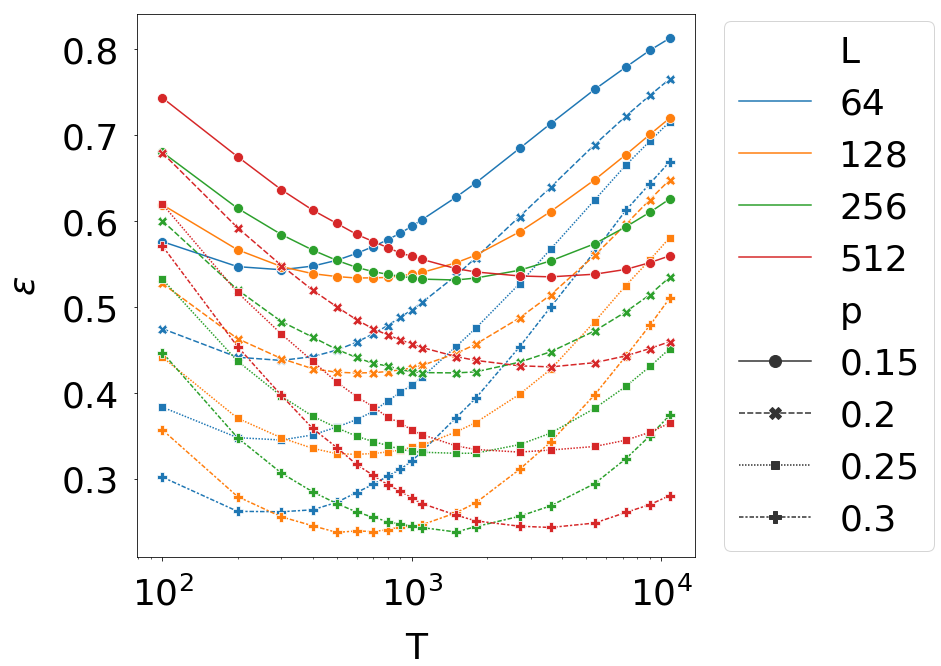
\includegraphics[width=\textwidth]{manna_t_267}
		\caption{Модель Манна, $\gamma=2.67$}
		\label{pic:manna_t_267}
	\end{subfigure}
	\begin{subfigure}[b]{0.45\textwidth}
		\centering
		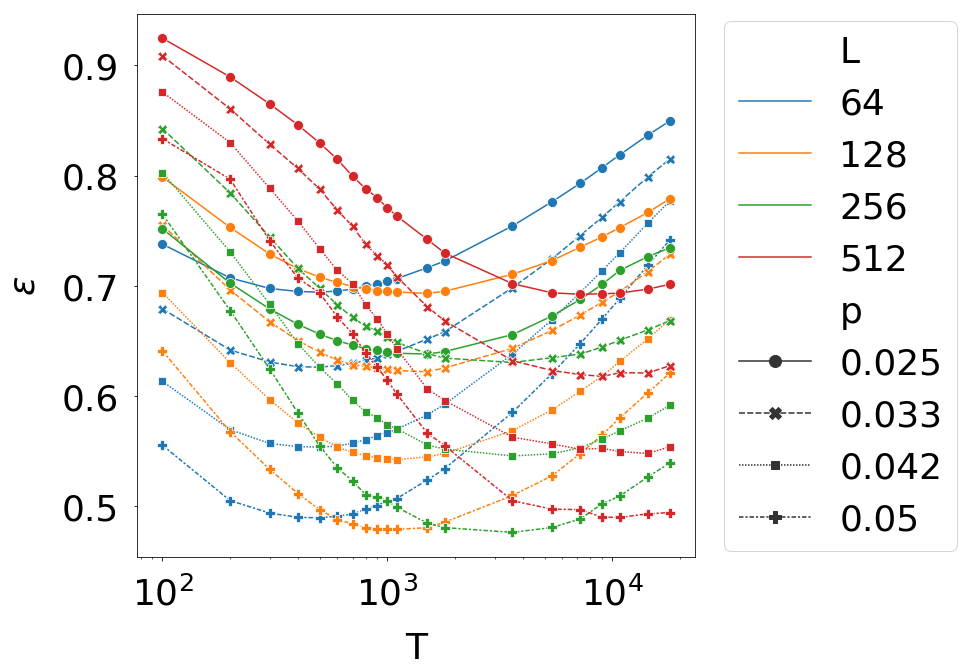
\includegraphics[width=\textwidth]{btw_t_293}
		\caption{Модель БТВ, $\gamma=2.93$}
		\label{pic:btw_t_293}
	\end{subfigure}
	\caption{Качество модели в зависимости от параметра $T$}
	\label{pic:t(L)}
\end{figure}

Формула для переменной принятия решения $y$ похожа на AR(1)-процесс. Поэтому мы ожидаем, что параметр $T$ отвечает за объем памяти в данной модели: чем больше память $T$, тем большее влияние имеет история предыдущих событий, что позволит увеличить качество модели. В то же время, слишком большая память может заставить алгоритм не делать акцент на последних событиях, из-за чего возможны потери в точности.

Численные эксперименты из Приложений \eqref{appendix:a} и \eqref{appendix:b} с разными параметрами $L$, $\gamma$ и $p$ подтвердили наше предположение  о влиянии параметра $T$. Форма кривой $\epsilon_{L, p, \gamma}(T)$ одинаковая для любых $L$, $\gamma$ и $p$ как в модели Манна, так и в модели БТВ, и имеет вид выпуклой функции с единственным пологим минимумом, как на Рис.~\eqref{pic:t(L)}. При том в модели Манна точка минимума не зависит от констант $p$ и $\gamma$, а зависит лишь от размера решетки $L$. Однако, в модели БТВ точка минимума зависит от $\gamma$ и остается независимой от $p$. Эмпирически мы пришли к выводу, что оптимальной $T(L)$ в модели Манна можно считать функцию $T(L) = 300 \cdot 2.25^{\log_{2}\frac{L}{64}}$, в модели БТВ для $\gamma=2.93$ функцию $T(L) = 500 \cdot 2.75^{\log_{2}\frac{L}{64}}$, а для $\gamma=3$ функцию $T(L) = 400 \cdot 2.5^{\log_{2}\frac{L}{64}}$.

\clearpage
\subsection{Скейлинг в модели Манна}

\begin{figure}[h]
	\centering
	\hspace{-25mm}
	\begin{subfigure}[t]{0.27\textwidth}
		\centering
		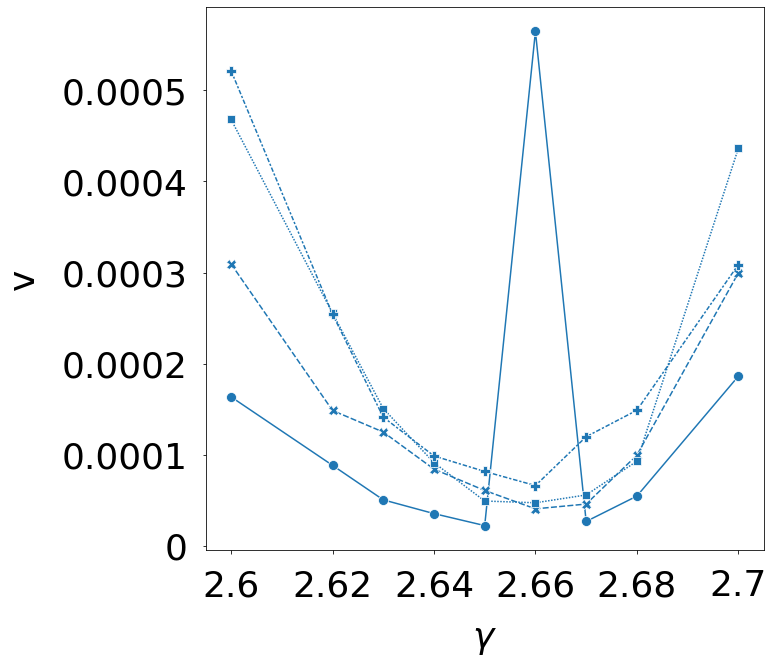
\includegraphics[height=\textwidth]{var_manna}
		\caption{Дисперсия}
	\end{subfigure}
	\hspace{10mm}
	\begin{subfigure}[t]{0.27\textwidth}
		\centering
		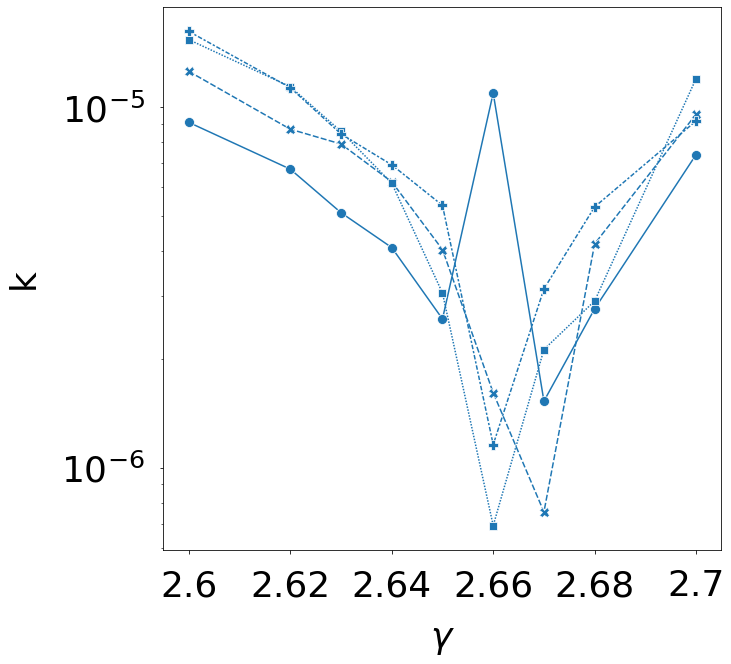
\includegraphics[height=\textwidth]{k_manna}
		\caption{Абсолютное значение коэффициента регрессирующей прямой}
	\end{subfigure}
	\hspace{10mm}
	\begin{subfigure}[t]{0.27\textwidth}
		\centering
		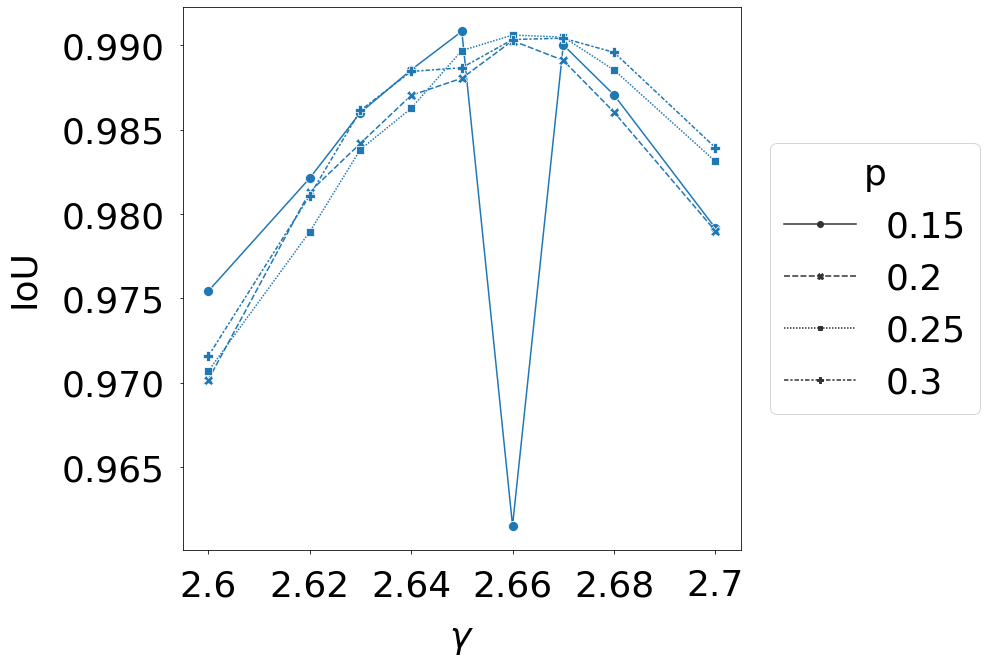
\includegraphics[height=\textwidth]{IoU_manna}
		\caption{IoU}
	\end{subfigure}
	\caption{Метрики качества шкалирования в модели Манна в зависимости от параметра $\gamma$}\label{pic:manna_scaling_metrics}
\end{figure}

Следующей серией численных экспериментов мы установили, что в модели Манна оптимальное $\gamma \approx 2.67$, что подтверждают все три метрики $v(\gamma, p)$, $k(\gamma, p)$ и $IoU(\gamma, p)$ на Рис. \eqref{pic:manna_scaling_metrics}. 

Однако более детальный анализ качества модели с параметром $\gamma = 2.67$ с помощью Рис. \eqref{pic:manna_t_267} показывает, что данный показатель для решетки $L=64$ слишком большой, а для решетки $L=512$ наоборот слишком маленький. Из этого можно сделать вывод, что $\gamma$ должна расти с ростом $L$. Мы считаем, что предельным показателем является $\gamma=2.75$, что согласовывается с показателем шкалирования плотности распределений событий в модели Манна. Дополнительно, мы хотим обратить внимание, что показатель шкалирования плотности распределений событий для таких малых решеток, как у нас, тоже имеет значение $2.67$, а не предельное $2.75$; это видно в экспериментах, отраженных в Приложении \eqref{appendix:d}.

\subsection{Скейлинг в модели БТВ}

\begin{figure}[h]
	\centering
	\centering
	\hspace{-25mm}
	\begin{subfigure}[t]{0.27\textwidth}
		\centering
		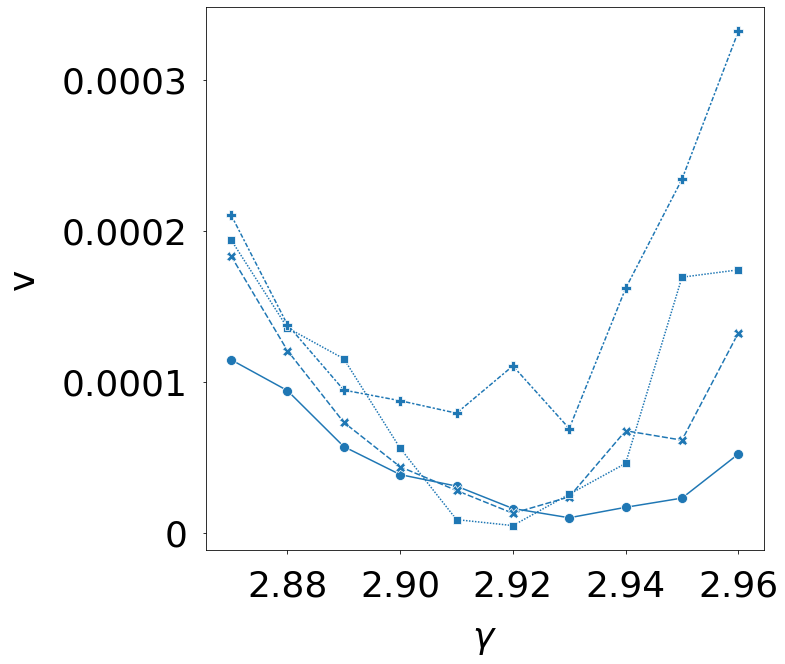
\includegraphics[height=\textwidth]{var_btw}
		\caption{Дисперсия}
	\end{subfigure}
	\hspace{10mm}
	\begin{subfigure}[t]{0.27\textwidth}
		\centering
		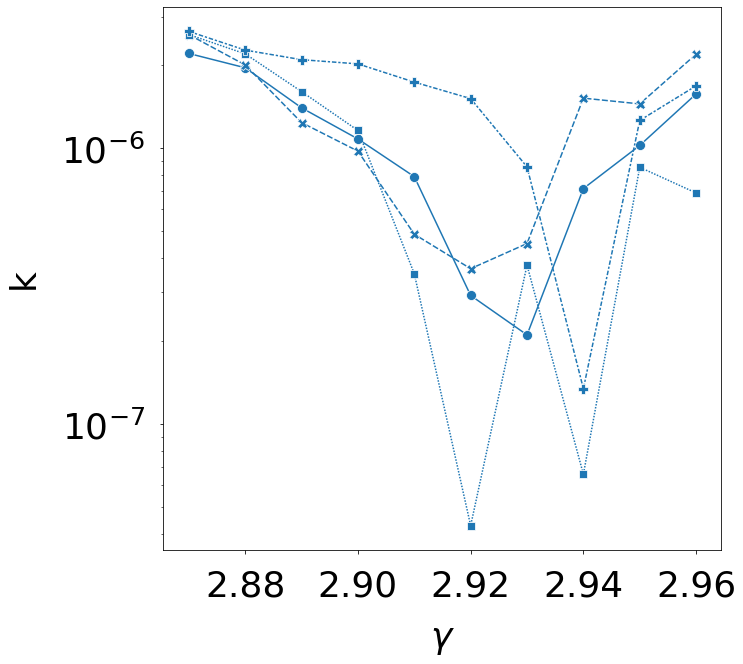
\includegraphics[height=\textwidth]{k_btw}
		\caption{Абсолютное значение коэффициента регрессирующей прямой}
	\end{subfigure}
	\hspace{10mm}
	\begin{subfigure}[t]{0.27\textwidth}
		\centering
		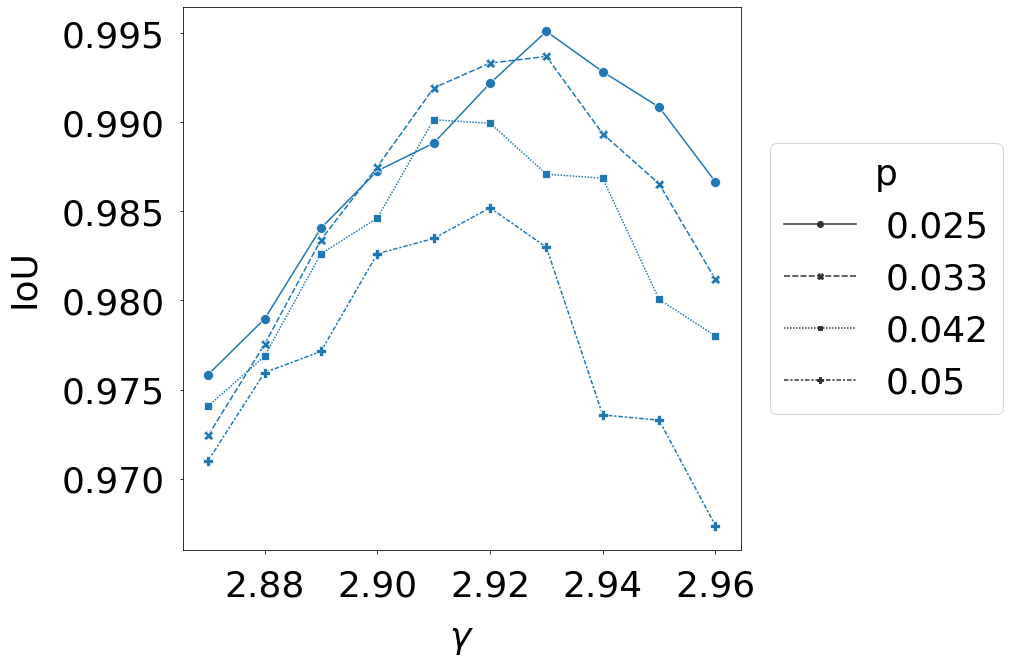
\includegraphics[height=\textwidth]{IoU_btw}
		\caption{IoU}
	\end{subfigure}
	\caption{Метрики качества шкалирования в модели БТВ в зависимости от параметра $\gamma$}\label{pic:btw_scaling_metrics}
\end{figure}

В модели БТВ нам удалось добиться аналогичных результатов: численные эксперименты на Рис. \eqref{pic:btw_scaling_metrics} показывают, что оптимальное $\gamma \approx 2.93$ по всем трем метрикам. Но согласно Рис. \eqref{pic:btw_t_293} мы видим, что для малых решеток показатель должен быть меньше, а для больших --- больше. В работе~\cite{Garber2009} авторы наблюдают такой же показатель для шкалирования размеров максимальных событий $s_{\max}$, и объясняют его эффектом конечного размера. Поскольку теоретическое значение максимального размера события пропорционально $L^3$, мы считаем, что предельным показателем шкалирования является $\gamma=3$.

\subsection{Качество прогноза}

\begin{figure}[h]
	\centering
	\begin{subfigure}[t]{0.45\textwidth}
		\centering
		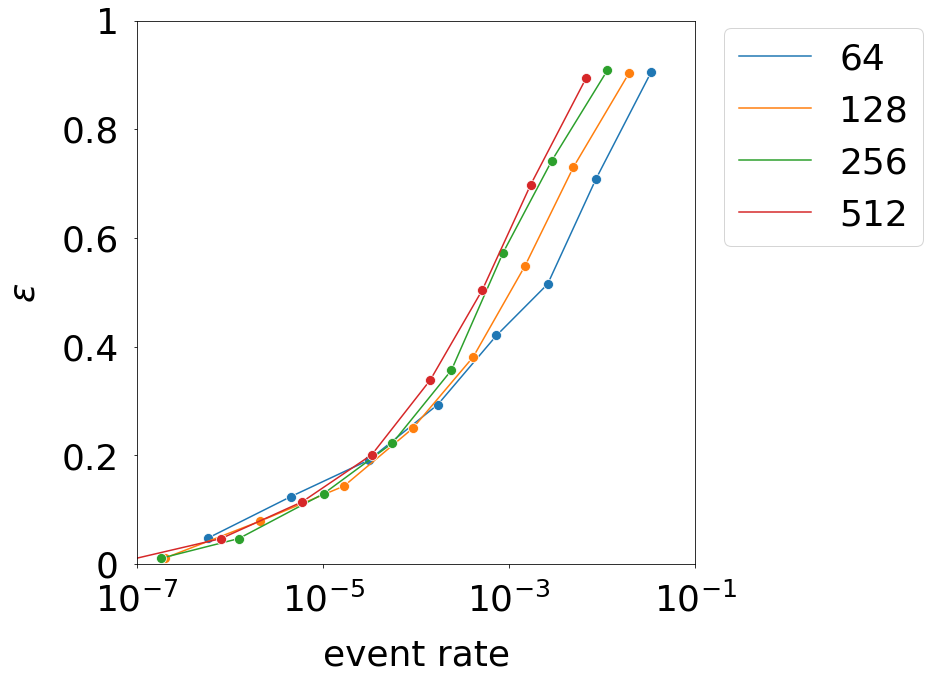
\includegraphics[width=\textwidth]{eps_vs_event_rate_manna}
		\caption{Модель Манна}
		\label{pic:event_rate_manna}
	\end{subfigure}
	\begin{subfigure}[t]{0.45\textwidth}
		\centering
		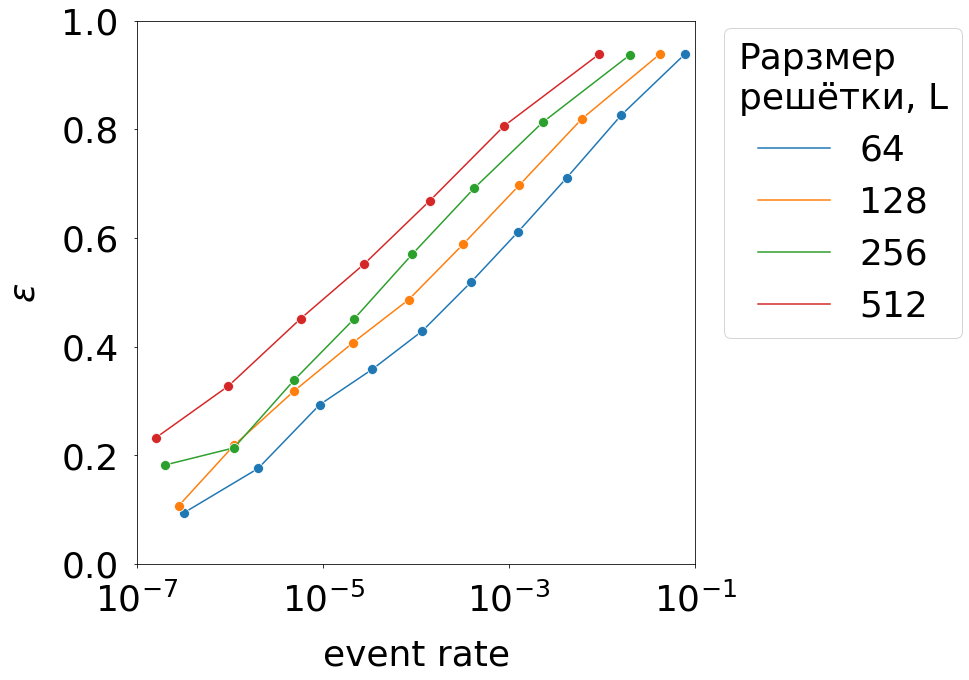
\includegraphics[width=\textwidth]{eps_vs_event_rate_btw}
		\caption{Модель БТВ}
		\label{pic:event_rate_btw}
	\end{subfigure}
	\caption{Качество прогноза в зависимости от частоты встречаемости событий}\label{pic:event_rate}
\end{figure}

Последним экспериментом мы хотели пронаблюдать качество прогноза $\epsilon$ в зависимости от частоты встречаемости событий $event\ rate$. Обратим внимание, что параметр $\gamma$ влияет лишь на качество скейлинга, и не влияет на график $\epsilon$ против $event\ rate$. Поэтому данная кривая является фундаментальным свойством нашего алгоритма прогнозирования критических событий.

\begin{figure}[h]
	\centering
	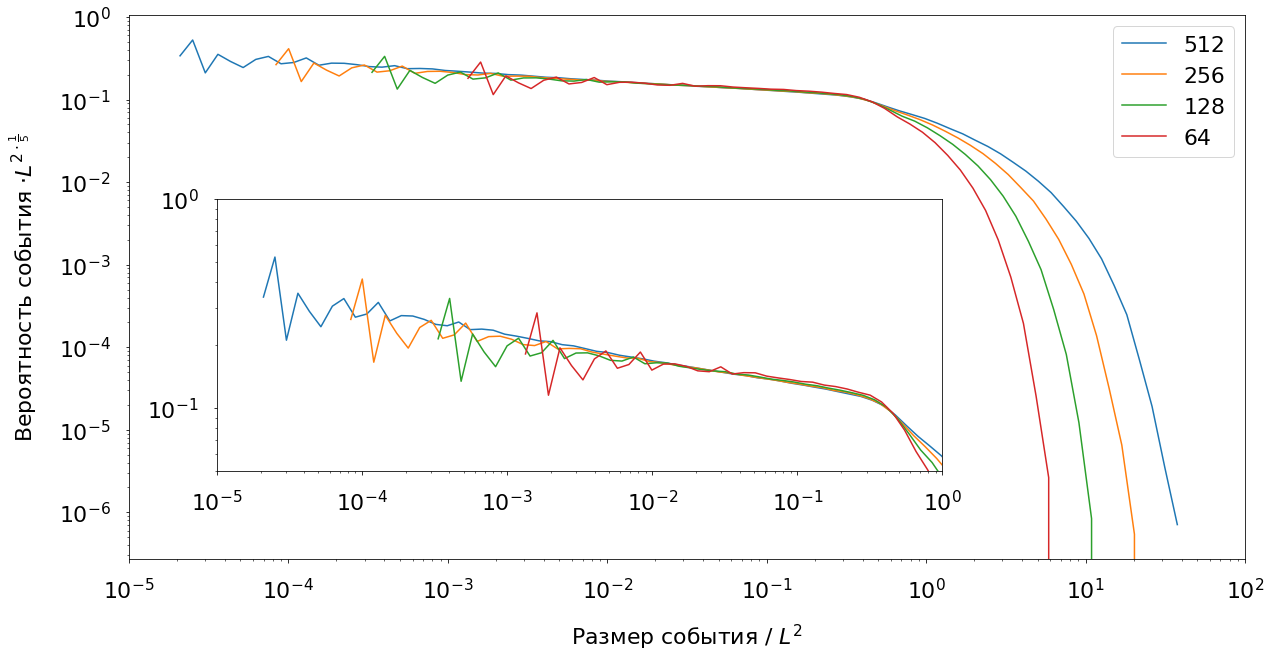
\includegraphics[width=\textwidth]{btw_distribution_200}
	\caption{Шкалирование степенной части в модели БТВ}\label{pic:btw_scaling}
\end{figure}

Результаты в модели Манна показывают, что для достаточно редких событий качество прогноза не зависит от размера решетки $L$. В то же время в модели БТВ качество прогноза падает с ростом $L$ и имеет экспоненциальную зависимость от частоты встречаемости событий. Мы предполагаем, что данный эффект объясняется шкалированием плотностей распределения событий: в модели Манна скейлинг полностью накладывает плотности распределений, как видно в Приложении~\eqref{appendix:d}. В то время как в модели БТВ крупные события, которые мы прогнозируем, шкалируеются как $L^3$, а основная степенная часть --- как $L^2$, что можно наблюдать на Рис.~\eqref{pic:btw_scaling}, и, как следствие, $event\ rate$ падает, если мы хотим сохранять одну и ту же эффективности прогноза с ростом $L$.
